\chapter{Sistema de grabación online}

Para poder obtener audios de distintas personas se desarrolló una página web. Esto nos da muchas ventajas ya que nos permite grabar fácilmente desde cualquier lugar. En esta sección explicaremos la arquitectura del sistema y sus detalles técnicos.

La página web esta desarrollada en Django versión 1.4.2 que es un framework para la creación de paginas web. Se eligió este framework por su facilidad a la hora de salvar objetos a la base de datos y también por la cantidad importante de librerías que posee Python. La versión utilizada de Python es 2.7.3. Esta misma necesita una base de datos para guardar cada clase de dominio. En esta base de datos vamos a guardar la información de cada hablante, las frases a grabar y las trazas principalmente. La base de datos utilizada fue PostgreSQL versión 9.1 y se eligió esta ya que es de código abierto. Los archivos de audio se van a grabar en archivos \textit{.wav} por separado y vamos a guardar una referencia al nombre del archivo generado en la base de datos. Para el servidor HTTP se utilizó Apache versión 2.2.22. El servidor corre en el sistema operativo Ubuntu 12.04.4 LTS.


\section{Requerimientos}

Los requerimientos son básicos: micrófono, conexión a internet. 
Tuvimos problemas sobre el browser que utilizaba. Wami necesita Flash versión 11.04 que no se encuentra en los repositorios tradicionales de Ubuntu. De esta manera, los navegadores que utilicen Flash instalado por el sistema operativo Ubuntu no podrán correr. Otros sistemas operativos, como Windows o IOs, no tienen problemas en la versión de Flash instalada. De todas formas el navegador Chrome posee preinstalado dicha versión de Flash, entonces este navegador puede correr perfectamente la aplicación sin importar el sistema operativo.

\section{Recolección de datos}

Cuando un usuario visita nuestra página, primero le hace llenar un formulario. Este le pregunta: género, fecha de nacimiento y de qué lugar es oriundo. Al confirmar los datos, estos son grabados en la base de datos de la aplicación en el servidor. Esto se puede apreciar en la Figura \ref{figEncuesta}. Luego se procede a realizar las grabaciones. 

\begin{figure}[h!]
    \centerline{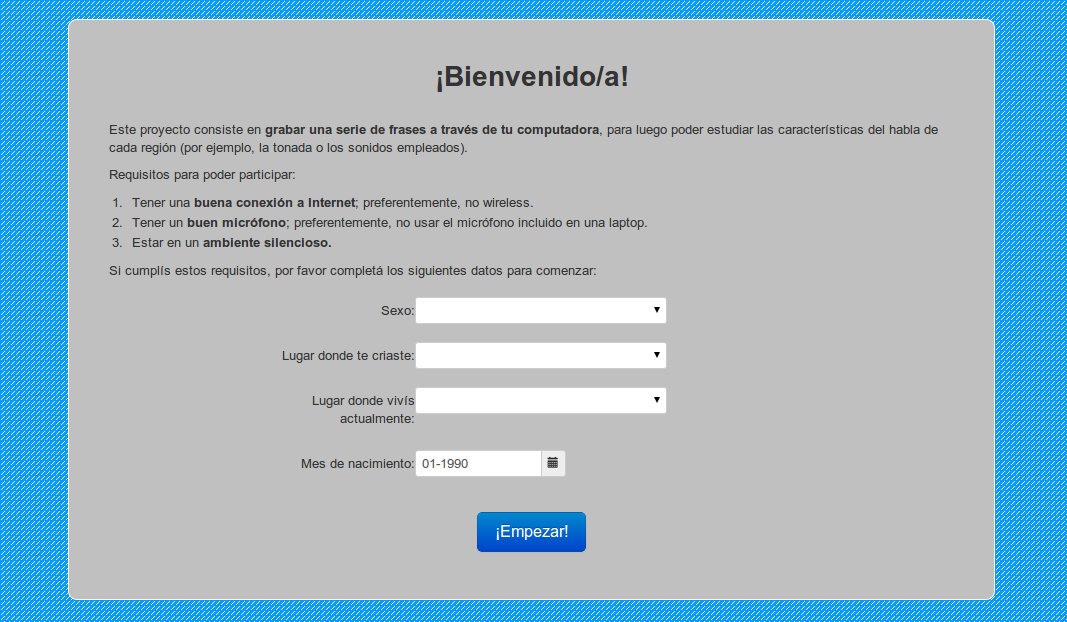
\includegraphics[width=0.7\textwidth]{pag-inicio2} }
    \caption{Encuesta inicial del sistema}
    \label{figEncuesta}
\end{figure}

\begin{figure}[h!]
    \centerline{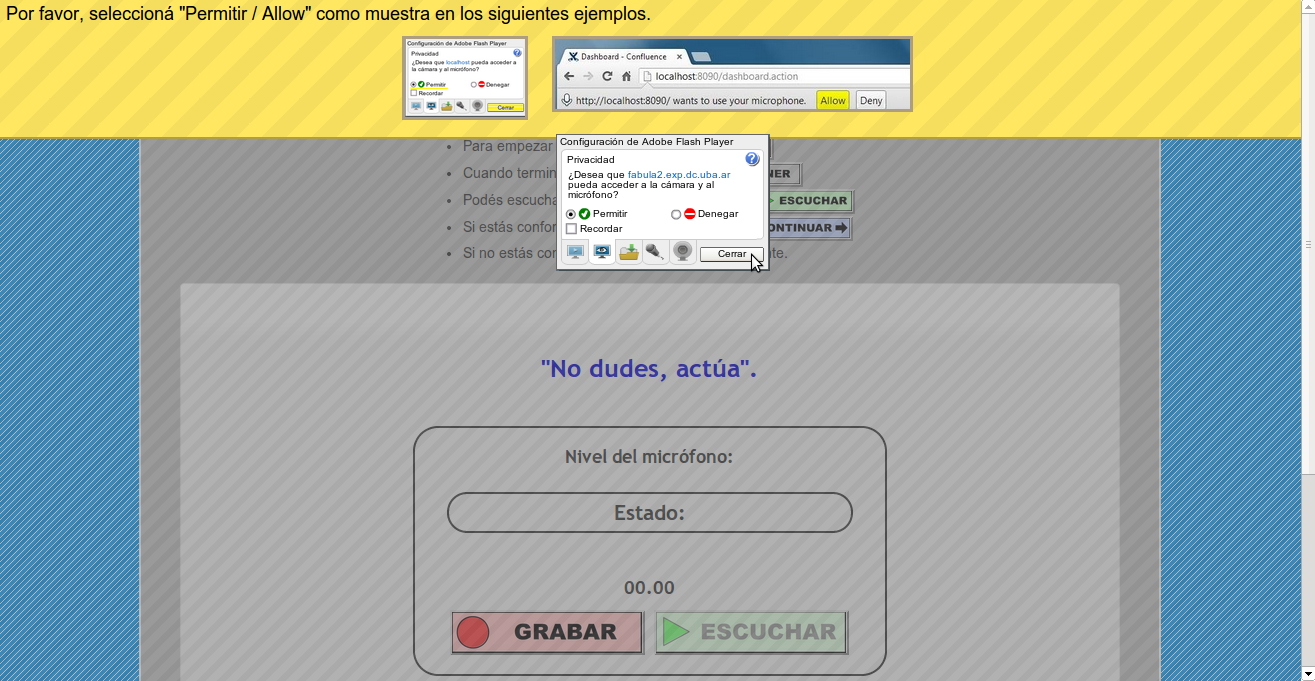
\includegraphics[width=0.7\textwidth]{pag-allow1} }
    \caption{Se debe permitir micrófono para comenzar el experimento}
    \label{allowmic}
\end{figure}

\begin{figure}[h!]
    \centerline{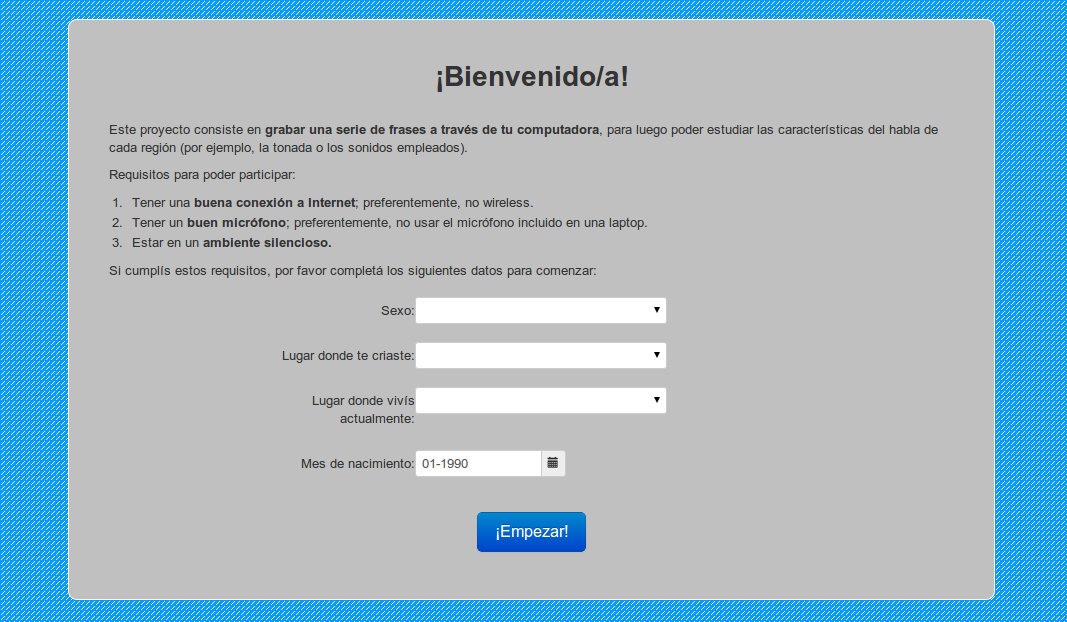
\includegraphics[width=0.7\textwidth]{pag-inicio2} }
    \caption{Inicio del experimento}
    \label{inicio}
\end{figure}

\begin{figure}[h!]
    \centerline{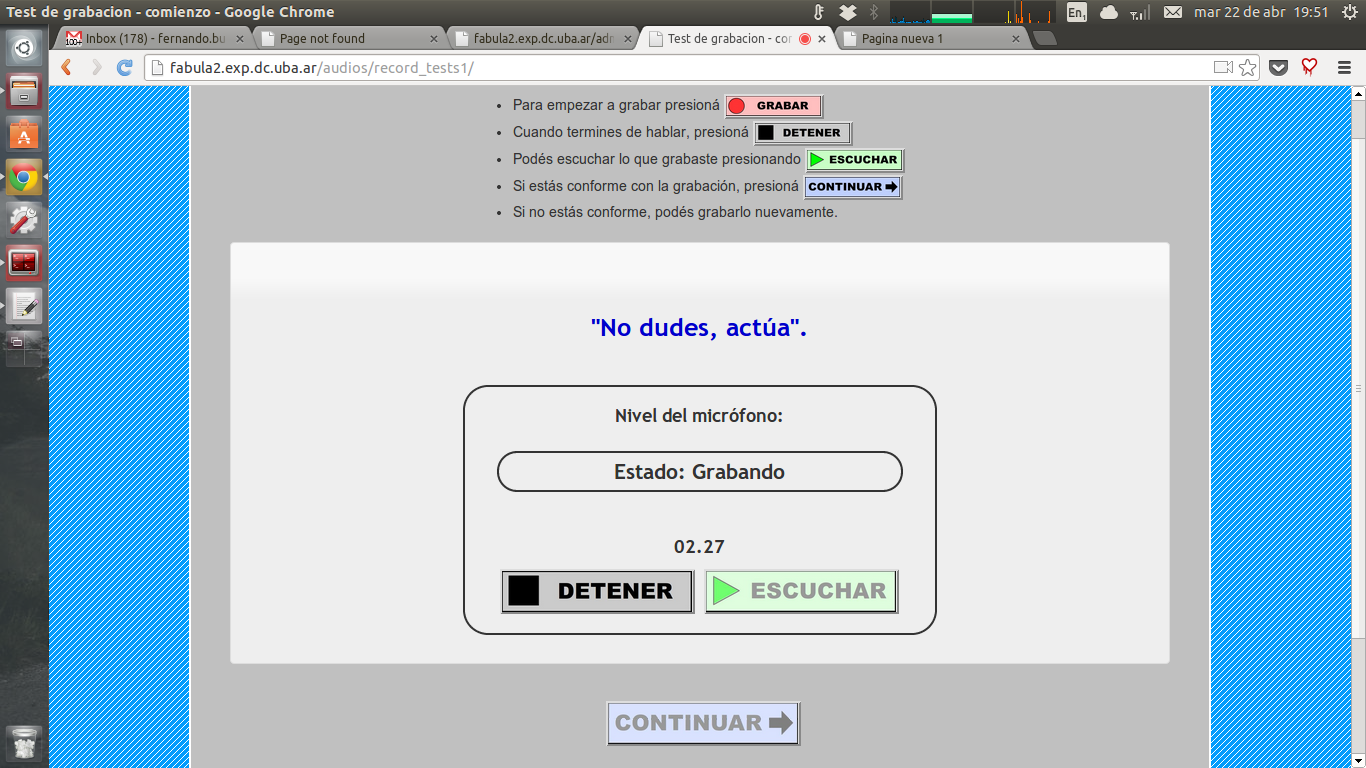
\includegraphics[width=0.7\textwidth]{pag-grabar1} }
    \caption{Grabando una frase}
    \label{grabando}
\end{figure}

\begin{figure}[h!]
    \centerline{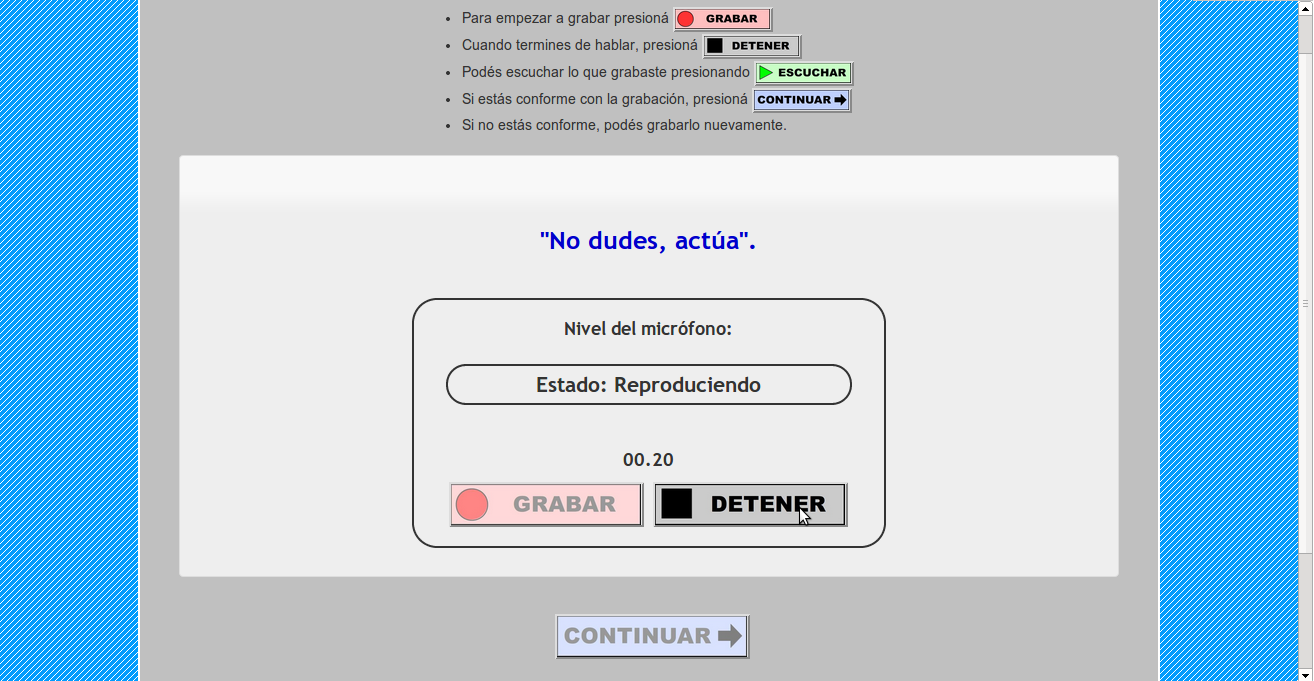
\includegraphics[width=0.7\textwidth]{pag-play1} }
    \caption{Reproduciendo la frase anteriormente grabada}
    \label{reproduciendo}
\end{figure}

En la pantalla de grabación el usuario deberá confirmar tener acceso al micrófono que posee en su dispositivo, como se puede ver en la Figura \ref{allowmic}.  Una vez hecho esto, se le explica las instrucciones (Fig. \ref{inicio}) y puede empezar a grabar. Cada nuevo experimento utiliza una nueva traza. El experimento en total consiste en realizar 40 grabaciones. El hablante va grabando de a 5 frases, cada vez que las termina de grabar ofrece la opción de seguir grabando otras 5 más. De esta forma, aporta el tiempo que puede. La interfaz que aprecia el usuario al grabar se puede ver en la Figura \ref{grabando}. Las grabaciones pueden ser escuchadas antes de ser confirmadas por el usuario. Lo importante es que la grabación se escuchen lo mejor posible. Para reproducir se aprieta en el botón \textit{Reproducir} como se ve en Figura \ref{reproduciendo}.

Cada vez que se confirma una grabación, esta se graba en un archivo wav en el servidor. El archivo wav que se genera tiene una frecuencia de muestreo de 22050 Hz y posee un sólo canal. Con estas características pudimos obtener un audio de calidad buena.

%todo: PONER DATOS TECNICOS DEL TIPO DE WAV

\section{Grabación a través del browser}

Los navegadores actuales no pueden soportar acceder al micrófono directamente. Durante la tesis, se desarrolla HTML5 que podrá soportar acceder al micrófono más fácil. No se eligió basarse en este porque sólo algunos browsers lo soportaban. Al ser un estándar muy nuevo necesita que el usuario tenga instalada últimas versiones de software y eso excluiría gente. Es por eso que debimos utilizar alguna tecnología alternativa. Buscando encontré un proyecto llamado WAMI que es una aplicación Flash que nos permite acceder al micrófono a través de JavaScript. 

El proyecto WAMI \footnote{http://code.google.com/p/wami-recorder/} nos permite acceder al micrófono de la computadora utilizando Flash. Este posee una interfaz que permite utilizar la aplicación Flash desde Javascript. De esta forma, no es necesario analizar en la implementación. Utilizando dicha interfaz se puede configurar varias urls. Una de ellas es donde envía la información de lo grabado.

Cuando termina de grabar, se envía un mensaje POST al servidor. Este obtiene el paquete de información y lo guarda como archivo .wav. Cuando se quiere reproducir algún audio se envía un mensaje GET a través de la interfaz. El servidor lo responde con el audio requerido y se reproduce en el navegador. 

Como se mencionó antes, para poder acceder al micrófono el usuario debe habilitar permisos para que la aplicación acceda al hardware de su computadora. Esto aparece como una ventana emergente al principio del experimento. Esto se puede ver en la Figura \ref{allowmic}. También se puede configurar la calidad del audio grabado y analizar el nivel del volumen que posee. Se guarda un registro de nivel de volumen sobre la interfaz para utilizar esos datos en algún proyecto futuro.

\section{Varias grabaciones por frase}

Siguiendo con la idea de tener la mejor grabación de cada hablante, le dimos la opción a cada hablante de que después de grabar un audio de una frase puedan escucharse como quedó. Esto requiere un ida y vuelta entre el cliente (navegador) y el servidor. Al grabar, el cliente manda un mensaje HTTP POST para el servidor con los datos de grabación. Las frases son de corta longitud entonces no es necesario preocuparse por la longitud del paquete. Cuando el cliente quiere escucharlo envía un mensaje GET a ese mismo audio anteriormente grabado. El servidor envía la grabación y es reproducida en el cliente. Esta ida y vuelta de la grabación podría ser optimizada para que la grabación pueda ser escuchada sin tener interacción con el servidor. En nuestro experimento, no tuvimos problemas graves en lo que respecta a latencias pero si es un punto débil del sistema.

A cada hablante le dimos la opción que pueda escuchar y volver a grabar la frase cuantas veces quisiera. Esto lo hicimos para poder detectar cual es el disparador que hace que diga mal una frase. Puede resultar interesante analizar los anteriores audios y porque se queda con el último.

\section{Sistema de administración}

El sistema debe tener datos precargados para estar activado recolectando hablantes. Los mínimos datos para poder tener la página funcionando en vivo son los datos de las trazas y la clasificación de los audios. Este cargo de datos se pueden guardar con fixtures del framework Django. Esta es un característica que nos permite guardar en un archivo datos para cargar antes de habilitar la web para estar online. Una vez cargado esos datos, los hablantes van a acceder a una url donde van a poder realizar el experimento grabando los distintos audios.

\subsection{Etiquetando audios}

Cuando varias personas terminan el experimento, los administradores pueden acceder a una url donde se puede escuchar cada audio que se va generando. Y si fue exitoso, o sea no esta saturado y no tiene ruidos, puede etiquetarlo con alguna de las etiquetas definidas. Las etiquetadas utilizadas esta vez son: ‘Conservar’,  ‘Sonido saturado’, ‘Mucho ruido de fondo’, ‘Problemas en el habla’. Más adelante veremos como obtener estos audios. Esto se puede ver en Figura \ref{cat}.

\begin{figure}[h!]
    \centerline{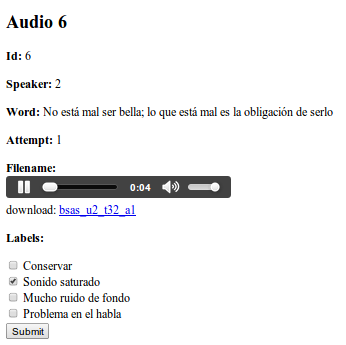
\includegraphics[width=0.5\textwidth]{categorizando_audios} }
    \caption{Categorizando audios}
    \label{cat}
\end{figure}

\paragraph{Backups automáticos}

El sistema posee backups automáticos generados a la noche automáticamente. Los backups consisten en un dump de la base de datos y de sincronizacion de los audios con una carpeta de backup. De esta forma, se guardan todos los datos cada día, y los audios quedan a salvo.

\paragraph{Export de wavs y csv}

Luego de obtener varios audios podemos exportar todos los datos a traves de urls. Utilizamos distintas urls que nos van a permitir bajarnos los audios etiquetados. Por ejemplo si accedemos a /conservados vamos a bajar los audios etiquetados de esa forma. Idem para las demas. Tambien se pueden bajar todos los audios sin etiquetas. Sobre la base de datos, se pueden bajar todo el modelo de datos a formato csv.

\section{Filtrado de audios}

Debemos evitar grabar audios saturados. Para ello se nos ocurrió medir el volumen de la grabación cuando sucede la misma. El resultado es una serie de valores entre 0 a 100. Sobre estos valores vamos a calcular el máximo y el mínimo. Si el primero es mayor a un cierto umbral (o sea mayor a 80) quiere decir que en la grabación se saturó en algún momento. Si el mínimo es menor a un cierto umbral (o sea menor a 20 por ejemplo) quiere decir que hay mucho sonido ambiente. En cualquiera de los dos casos podemos pedirle al usuario que grabe devuelta el experimento. De esta forma podemos filtar audios que no nos servirán para reconocer el acento.

Si bien esta característica esta fue programada, no fue utilizada en la recolección de datos. El motivo fue que queríamos chequear cuan bien funcionaba la herramienta sin filtros y con completa participación de los usuarios. Otro motivo fue la paciencia de los hablantes. Puede suceder que al tratar de grabar no logre un ambiente beneficioso para grabar. Esto quiere decir que aunque quiera grabar el filtro rechace todos sus audios. También notamos que había grabaciones que dieron mal el filtrado del volumen pero la grabación era buena. Esto no lo queremos como primer experimento del framework. Por eso elegimos aceptar todos sus audios.

Para los audios que salieron saturados, más adelante vamos a realizar un estudio para intentar sacarles el ruido y de esta forma intentar rescatarlos.
